% %%%%%%%%%%%%%%%%%%%%%%%%%%%%%%%%%%%%%%%%%%%%%%%%%%%%%%%%%%%%%%%%%%%%%%%%%%%%%
% %%%%%%%%%%%%%%%%%%%%%%%%%%%%%%%%%%%%%%%%%%%%%%%%%%%%%%% Building on Mann 1995
% %%%%%%%%%%%%%%%%%%%%%%%%%%%%%%%%%%%%%%%%%%%%%%%%%%%%%%%%%%%%%%%%%%%%%%%%%%%%%

\chapter{Results}
  \label{ch_results}

\todo{This chapter is the real moneymaker. The overarching motivation for this work is that Pc4 pulsations vary in interesting ways with respect to azimuthal modenumber, and that prior models have been unable to give a good picture of that behavior. }

%\todo{Do we every check E/B against $\Sigma_P / \mz$? }

%\todo{Do we see a difference between \vec{k} (momentum) and the group velocity? Poynting flux will always be pretty much along the field line, since $B_3$ is small and $E_3$ is zero, but the wave vector need not be. This is a question of coupling/converting to compressional waves, I guess. }

%\todo{Look at McKenzie and Westphal. Waves incident on the bow shock, etc, at weird angles. }

%\todo{Look at the E to B ratio. Compare to the \Alfven speed and to the height-integrated Pedersen conductivity. }

% =============================================================================
% =============================================================================
% =============================================================================
%\section{Electromagnetic Energy Gap}

%\todo{A preliminary search (and asking Bob) has not turned up anyone looking at this before, so it's hard to provide context. }

%Above, we considered the decay of energy from the poloidal mode to the toroidal mode. A natural follow up is, are there any other surprising trends in the distribution of energy?

%As it turns out, yes!

%In cases where the driving frequency does not line up with the local bounce frequency, energy doesn't accumulate particularly well in either the poloidal or the toroidal mode. Like a damped-driven oscillator, the system's behavior follows the input. 

%At low \azm, what energy there is divides itself more or less equally between the electric and magnetic fields. 

%As \azm increases, oddly, a gap appears. When the conductivity is high, the magnetic field holds more energy than the electric field. The disparity can be up to a factor of $\sim \num{3}$; that is, \SI{75}{\percent}. of the energy in the magnetic field, and \SI{25}{\percent} in the electric field. When conductivity is low, the opposite happens: energy concentrates in the electric field. 

%This lines up somewhat with what might be expected. When conductivity is low, it takes a larger electric field to induce the same current, and thus the same magnetic field. But it's not clear why this disparity only appears at large \azm, or why it does not appear when the driving is resonant. 

%Maybe it's a timing issue? A relationship between the bounce time (which is more or less indepedent of \azm) and the rotation time (which depends on \azm). 

%\todo{How is the compressional magnetic field brought into these calculations? It exists only at small \azm. It's never particularly large, it also gets added to the zeroth-order field before squaring. }

%\begin{figure}[H]
%    \centering
%    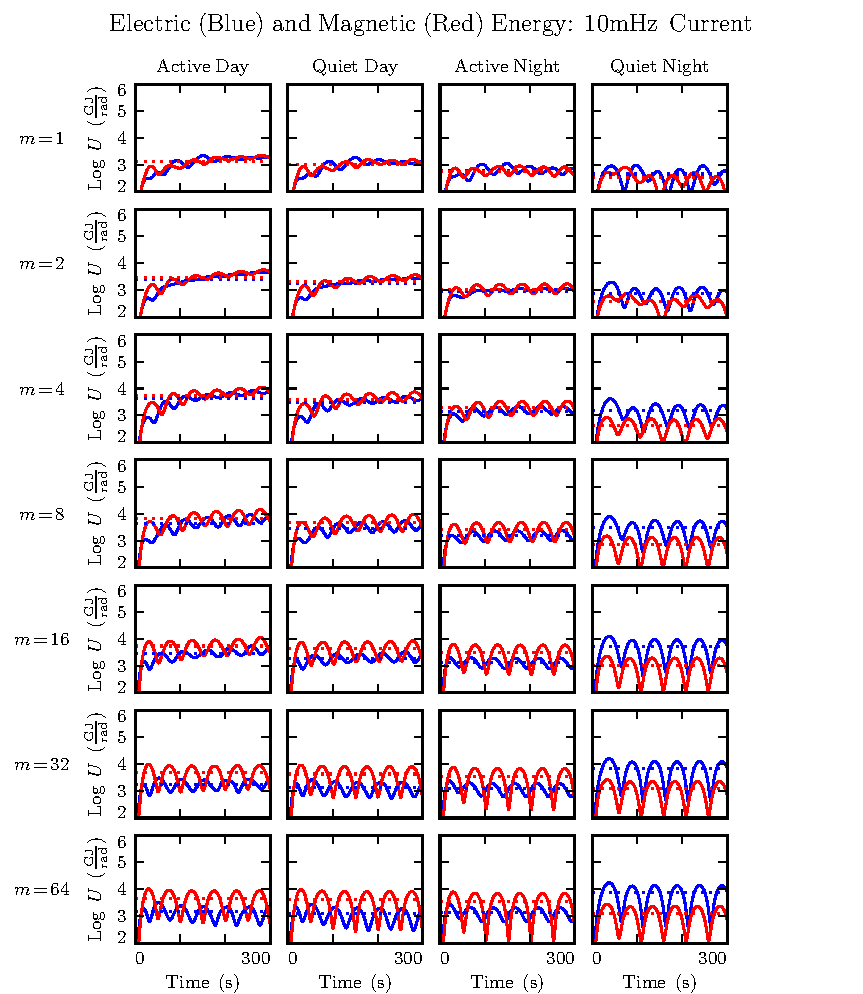
\includegraphics[width=\textwidth]{figures/U_BE_010mHz.pdf}
%    \caption[Current-Driven Electric and Magnetic Energy: 10mHz]{
%      In the absence of resonant driving, a disparity emerges at large \azm between the energy in the magnetic field and the energy in the electric field. The sign of the difference depends on the ionospheric conductivity. 
%    }
%    \label{fig_U_BE_010mHz}
%\end{figure}

%\begin{figure}[H]
%    \centering
%    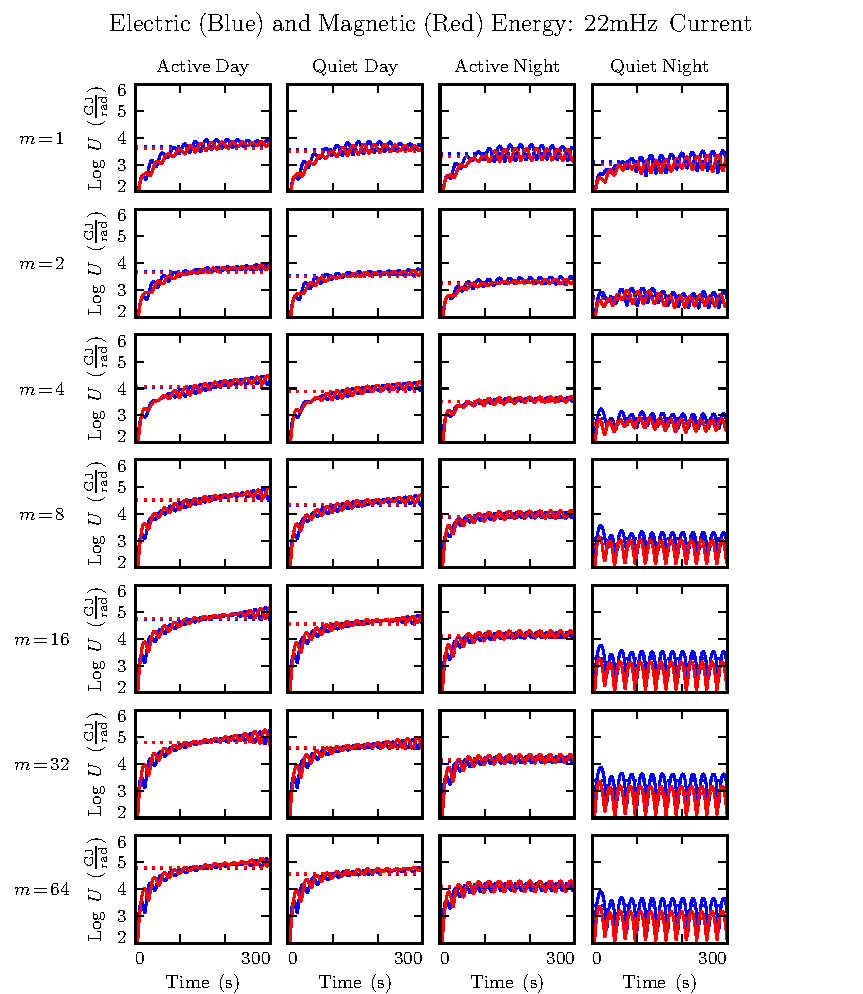
\includegraphics[width=\textwidth]{figures/U_BE_022mHz.pdf}
%    \caption[Current-Driven Electric and Magnetic Energy: 22mHz]{
%      When driving is resonant, energy is distributed almost exactly half-and-half between the electric and magnetic fields, regardless of \azm. The rightmost profile still shows a gap, likely because the ionospheric conductivity in that model is low enough that nothing ever resonates. 
%    }
%    \label{fig_U_BE_022mHz}
%\end{figure}












